\documentclass[a4paper,12pt]{hitec}
\usepackage[english]{babel}
\usepackage{etex}
\usepackage{times}
\usepackage{setspace}
\usepackage{inputenc}
\usepackage{amssymb}
\usepackage{amsfonts}
\usepackage{amsmath}
\usepackage{graphicx}%[pdftex]
\usepackage{wrapfig}
\usepackage{subfig}
\usepackage{alltt}
\usepackage{moreverb}
%for more info on hyperref package see http://en.wikibooks.org/wiki/LaTeX/Packages/Hyperref
%\usepackage[pdftex,colorlinks=true,linkcolor=blue]{hyperref}
\usepackage{eso-pic}
% tikz related packages to provide scalable graphics 
\usepackage{tikz}
\usetikzlibrary{mindmap,backgrounds}
\usepackage{lipsum}

\newcommand\BackgroundPic{
\put(0,-230){
\parbox[b][\paperheight]{\paperwidth}{%
\vfill
\centering

\includegraphics[width=\paperwidth,height=\paperheight, keepaspectratio]{sections/01-intro/images/00-splash}%
% \begin{tikzpicture}[mindmap, opacity=.4, scale=0.8, outer sep=0pt, transform shape,		    
% 		    level 2 concept/.append style={level distance=130, sibling angle=20}]
% 
%   \begin{scope}[mindmap, concept color=green!50, text=green!50!black, level 1 concept/.append style={level distance=130, sibling angle=35}]
%     \node [concept] at (-1.0, 2.0) (is) {Information Systems}[clockwise from=200] 
%       child {node [concept] (log) {Domain Models}}
%       child {node [concept] (alg) {Data Management}}
%       child {node [concept] (log) {User Interface}}
%       child {node [concept] (img) {Web Communication}}
%       child {node [concept] (opt) {Analysis and Reporting}}
%       child {node [concept] (res) {Security}};
%   \end{scope}
% 
%   %\node (dev) at (2.1,-4) [circle, minimum size=4cm,fill,draw,thick,color=red!50, text=red!50!black] {Developers};
%   \begin{scope}[mindmap, concept color=red!50, text=red!50, level 1 concept/.append style={level distance=140}, sibling angle=360]
%     \node [concept] at (3.1,-4) (dev) {Developers}[clockwise from=150] 
%       child {node [concept] (ide) {IDE}}
%       child {node [concept] (req) {Requirements Managment}}
%       child {node [concept] (dom) {Domain Modeling}}      
%       child {node [concept] (src) {Source Version Control}};
%   \end{scope}
% 
%   \begin{scope}[mindmap, concept color=blue!50, text=blue!50!black, level 1 concept/.append style={level distance=130, sibling angle=35}]
%     \node [concept] at (0.2,-10.0) (bus) {Business Requirements}[clockwise from=-5] 
%       child {node [concept] (accbud) {Accounting and Budgeting}}
%       child {node [concept] (ship) {Shipments}}
%       child {node [concept] (ord) {Ordering Products}}
%       child {node [concept] (work) {Work Orders}}      
%       child {node [concept] (hum) {Human Resources}};
%   \end{scope}
% % 
% % Connections 
%   \path (bus) to[circle connection bar switch color=from (blue!50) to (red!50)] (dev);
%   \path (dev) to[circle connection bar switch color=from (red!50) to (green!50)] (is);
% \end{tikzpicture}
\vfill
}}}


\begin{document}
 \AddToShipoutPicture*{\BackgroundPic}
  \setstretch{1.2}
  \begin{titlepage}
\title{Trident Genesis Platform Architecture from Engineering Perspective}
\company{Fielden Management Services Pty. Ltd.}
\author{TG Team}
\date{Lviv-Melbourne, 2011}
\maketitle
\clearpage
  This article provides a high level overview of the motivation, principle approaches and core features of the Trident Genesis software platform.
  The main emphasis is made on architectural and technological innovations, which together define a unique technology for the development and reliability improvement of business oriented applications.

\clearpage
\tableofcontents
\clearpage

\end{titlepage} % this file contains the title page and the abstract  
  \setcounter{page}{4} % need to reset page counter as by default after toc it start with 1 again 
  % using \input insterad of \include in order not statr every section from new page
  % need to include an image of the business rules to mind to code transition
\section{Motivation -- the ``why'' behind Trident Genesis}\label{sec:01}
  Software information systems\footnote{
    In this article the terms \emph{information system} and \emph{software application} are used interchangeably.
  } 
  (IS) are ubiquitous in modern society, which makes the ability to create and maintain reliable software critical from both consumer and manufacturer perspectives.
  The ideas and facilities built into a software application fully determine its purpose and value to the consumer (end user).
  That's why the subject of this article is the technological innovations, which are combined to provide a unique technology for the development of reliable business oriented information systems -- the Trident Genesis Platform (TG).

  \begin{wrapfigure}{r}{80mm}
    \centering    
    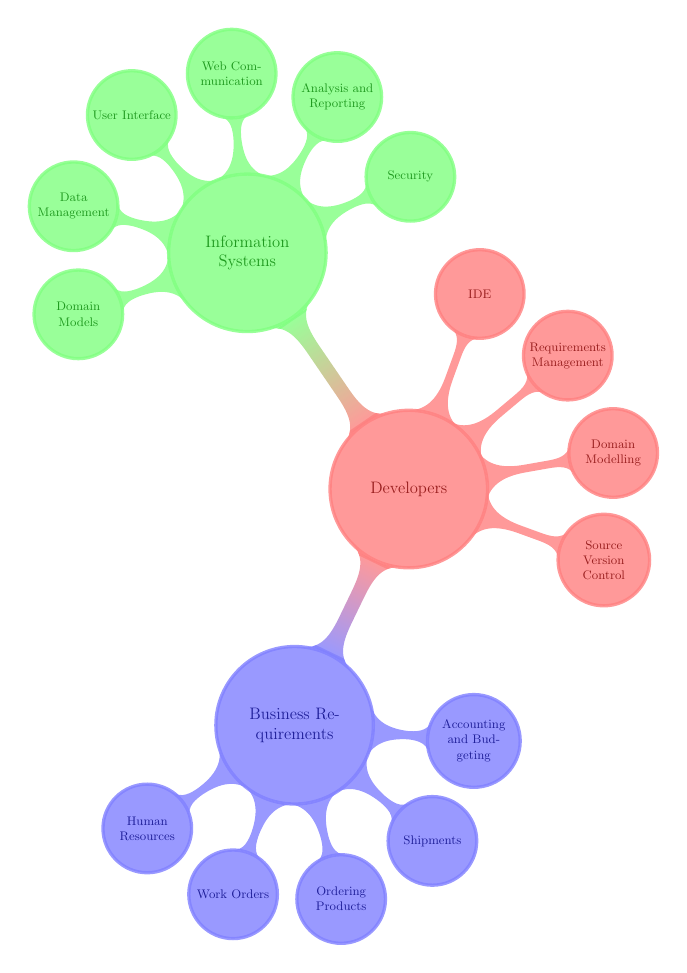
\begin{tikzpicture}[mindmap, opacity=0.8, scale=0.5, outer sep=0pt, transform shape]

      \begin{scope}[mindmap, concept color=green!50!white, text=green!50!black, level 1 concept/.append style={level distance=130, sibling angle=35}]
	\node [concept] at (-1.0, 2.0) (is) {Information Systems}[clockwise from=200] 
	  child {node [concept] (log) {Domain Models}}
	  child {node [concept] (alg) {Data Management}}
	  child {node [concept] (log) {User Interface}}
	  child {node [concept] (img) {Web Communication}}
	  child {node [concept] (opt) {Analysis and Reporting}}
	  child {node [concept] (res) {Security}};
      \end{scope}

      %\node (dev) at (2.1,-4) [circle, minimum size=4cm,fill,draw,thick,color=red!50, text=red!50!black] {Developers};
      \begin{scope}[mindmap, concept color=red!50, text=red!50!black, level 1 concept/.append style={level distance=150, sibling angle=30}]
	\node [concept] at (3.1,-4) (dev) {Developers}[clockwise from=70] 
	  child {node [concept] (ide) {IDE}}
	  child {node [concept] (req) {Requirements Management}}
	  child {node [concept] (dom) {Domain Modelling}}      
	  child {node [concept] (src) {Source Version Control}};
      \end{scope}

      \begin{scope}[mindmap, concept color=blue!50, text=blue!50!black, level 1 concept/.append style={level distance=130, sibling angle=35}]
	\node [concept] at (0.2,-10.0) (bus) {Business Requirements}[clockwise from=-5] 
	  child {node [concept] (accbud) {Accounting and Budgeting}}
	  child {node [concept] (ship) {Shipments}}
	  child {node [concept] (ord) {Ordering Products}}
	  child {node [concept] (work) {Work Orders}}      
	  child {node [concept] (hum) {Human Resources}};
      \end{scope}
    % 
    % Connections 
      \path (bus) to[circle connection bar switch color=from (blue!50) to (red!50)] (dev);
      \path (dev) to[circle connection bar switch color=from (red!50) to (green!50)] (is);
    \end{tikzpicture}
  \end{wrapfigure}

  First of all, it is important to understand what motivated the creation of TG and thus determined its main purpose.
  The evolution of computers led to an increase in computational power, which facilitated a significant increase in the amount of data that can be processed, and at the same time led to a need for a higher level of abstractions when creating software applications.
  Programming languages are at the core of software development, which also evolved -- from machine and assembly languages to modern mainstream programming languages such as Java, Scala, C\#.
  However, due to their nature all programming languages are convenient for instructing the computers how to perform specific computations, but not convenient for describing (modelling) the actual problem domain of the business being automated\footnote{Business for which an information system is being created.}.
  
  This leads to a huge semantic gap between the business requirements (what needs to be solved) and the actual solution (information system), which constitutes itself as a set of instructions to the computer.
  The two sides of the gap are bridged only by the software developers who have built the solution and hold the transition model in their minds.
  So the software developers serve as translators between the language of the business domain and the language of the software information system.
  Due to this and the fact that the same business requirements can be expressed in multiple ways using a general purpose programming language, there are many problems maintaining the solution, especially when the original developers are not around.

  In his paper ``Language Oriented Programming'', M.~P.~Ward points to several important research results:
  \begin{itemize}
    \item There is a thin spread of domain knowledge among software developers in most projects;    
    \item Most development is maintenance. 
	  System evolution is so common, that development from scratch is the exception rather than the rule;
    \item Most specifications are incremental. 
	  The customer is rarely able to provide a complete specification at any stage of the project;
    \item Domain knowledge is important;
    \item There is a gulf between developer and user. 
	  Few developers have adequate knowledge about the user's work. 
	  This leads to major misconceptions about the system's purpose.
  \end{itemize}
  
  To date most of the development of business applications involves low-level technical details, which deprive developers of the time to think and work on the actual business requirements.
  
  The above problems and our own experiences of having to deal with them on a daily basis led to the need of raising the level of abstraction that would hide low-level technical details and provide a uniform programming model for implementing software solutions as close as possible to the business terminology.
  By raising the level of abstraction the TG platform brings closer together software developers and business domain specialists, which is one of the platform's less obvious but defining features.
 % this file contains the first section of the docyment with all subsections
  \section{Types and Metadata == Business Modeling}\label{sec:02}

  In recent years there was a spike in popularity of the Domain-Specific Languages (DSL) concept, which can be explainded by the programming issues outlined in the introduction, which affect not only the business oriented information systems, but also other domains dependent on various informations systems.

  The concept of DSL is not new.
  In fact, there are well established solutions for business software what exist for a long time and explictly utilise this concept.
  For example, SAP Business Suite offers a specialised language ABAP and Microsoft Dynamics Axapta provides X++.
  These are examples of so called \emph{external DSL}, which are separate or external to the programming language used natively for creation of the mentioned products.
  The main disadvantage with external DSLs is this: if there is a need to express a complex algorithm the expressive power of a DSL should be adequate to implement such algorithm, which in turn makes that DSL yet another general purpose programming language.
  
  An opposite to external DSL is the concept of \emph{interna DSL} -- a specialised language, which utilises the capabilities of a specific general purpose programming language of expressing language-like constructs that can be used together with the general purpose programming language.
  Internal DSLs share the development and execution infrastructure of the corresponding general purpose programming language taking a significant advantage of reusing debugging, profiling tools, code editors, existing programming libraries etc.
  
  Different general purpose programming languages provide different degrees of support for developing sophisticated internal DSLs.
  For example, scripting languages generally provide better ways of implementing internal DSLs (e.g. Ruby).
  However, in our strong oppinion statically type langugages are of essential importantce for constructing complex business oriented information systems.
  
  From the very beginning the Trident Genesis Platform was envisaged as an application platform founded on the concept of internal DSLs and domain-driven development.
  It was decided to tap into the power of modern IDEs and existing programming skills of software developers, which resulted in the choice of Java as the host general purpose programming language\footnote{Java does not provide the best support for developing internal DSLs (e.g. Scala is a lot more adequate), but the maturity of the existing Java infrastructure and development experience played a critical part in this decision.}.

%   \begin{figure}[!htp]
%     \centering
%     
\includegraphics[width=10cm]{sections/01-intro/images/00-splash.jpg}
%     \caption{Example of an Embedded Image}\label{fig:01}
%   \end{figure}


%  // calculates the average yearly maintenance cost (for the last 3 years) per sectors of NORTH division. Only vehicles of MERCEDES make and models starting from 315 or 316 or VITO model are taken into account.
%         select(WorkOrder.class).
%         where(). //
%         prop("vehicle.model.make.key").eq().val("MERCEDES").and().
%         begin().prop("vehicle.model.key").starts_with().any_of_values("315", "316" ).or().prop("vehicle.model.key").eq().val("VITO").end().and().
%         year_of().prop("actualStart").in().values(2009, 2010, 2011).and().
%         prop("vehicle.station.zone.sector.division.key").eq().val("NORTH").
%         yield_and_group().prop("vehicle.station.zone.sector").as("sector").
%         yield().begin_expr().sum_of().prop("actualCost").div().val(3).end_expr().as("averageYearlyMaintenanceCostPerSector").model_as_aggregate();
  % use comments for providing useful information about document structure and content
\end{document}